% !TEX root = saveliev_physics_general_course_1.tex
%!TEX TS-program = pdflatex
%!TEX encoding = UTF-8 Unicode


\chapter{DYNAMICS OF A POINT PARTICLE}\label{chap:2}

\section{Classical Mechanics. Range of Its Applicability}\label{sec:2_1}

Kinematics describes the motion of bodies without being concerned with why a body moves exactly in a given way (for example, uniformly along a circle, or with uniform acceleration along a straight line), and not in a different one. 

Dynamics studies the motion of bodies in connection with its causes (the interactions between bodies) resulting in the occurrence of a specific kind of motion.

The so-called classical or Newtonian mechanics is based on three laws of dynamics that were formulated by Isaac Newton in 1687.

Newton's laws (like all other laws of physics) were the result of generalizing a great amount of experimental facts. Their correctness (although it covers a very extensive range of phenomena, the latter are nevertheless limited) is confirmed by the agreement of the corollaries following from them with experimental results.

Newtonian mechanics achieved such great successes during two centuries that many physicists of the 19th century were convinced in its omnipotence. It was considered that the explanation of any physical phenomenon required its reduction to a mechanical process obeying Newton's laws. With the development of science, however, new facts were uncovered for which no place could be found within the confines of classical mechanics. These facts were explained in new theories---the special theory of relativity and quantum mechanics.

The special theory of relativity advanced by Albert Einstein in 1905 radically revised Newton's notions of space and time. This revision resulted in the creation of ``high-speed mechanics'' or, as it is called, relativistic mechanics. The new mechanics did not result, however, in complete negation of the old Newtonian mechanics. The equations of relativistic mechanics in their limit (for speeds small in comparison with the speed of light) transform into the equations of classical mechanics. Thus, classical mechanics has entered relativistic mechanics as a particular case of it and has retained its previous significance for describing motions occurring at speeds much smaller than that of light.

Matters are similar with the relation between classical and quantum mechanics. The latter took root in the twenties of the present century as a result of the development of physics of the atom. The equations of quantum mechanics also result in those of classical mechanics in their limit (for masses that are great in comparison with the masses of atoms). Consequently, classical mechanics is also a part of quantum mechanics and is a limiting case of it.

Thus, the development of science has not eliminated classical mechanics, but has only shown its limited applicability. Classical mechanics based on Newton's laws is the mechanics for bodies of large (compared with the mass of atoms) masses travelling at low (compared with the speed of light) speeds.

\section{Newton's First Law. Inertial Reference Frames}\label{sec:2_2}

Newton's first law is formulated as follows: \textit{every body continues in its state of rest or of uniform motion in a straight line unless it is compelled by external forces to change that state}. Both states named are distinguished by the acceleration of the body equalling zero. Therefore, the first law can also be formulated as follows: the velocity of every body remains constant (in particular, it equals zero) until the action of other bodies on this body causes it to change.

Newton's first law is obeyed not in any reference frame. We have already noted that the nature of motion depends on the choice of the reference frame. Let us consider two frames of reference moving with respect to each other with a certain acceleration. If a body is at rest relative to one of them, then it will obviously travel with acceleration relative to the other one. Consequently, Newton's first law cannot be obeyed simultaneously in both frames.

A reference frame in which Newton's first law is obeyed is called an \textbf{inertial} one. The law itself is quite often called the \textbf{law of inertia}. A reference frame in which Newton's first law is not obeyed is called a non-inertial reference frame. There is an infinite multitude of inertial frames. Any reference frame moving uniformly in a straight line (\ie, with a constant velocity) relative to an inertial frame will also be an inertial one. This will be discussed in greater detail in Sec.~\ref{sec:2_7}.

It has been established experimentally that the reference frame whose centre coincides with the Sun and whose axes are directed toward appropriately selected stars is an inertial one. This system is defined as a \textbf{heliocentric reference frame} (\textit{helios} means Sun in Greek). Any reference frame moving uniformly in a straight line relative to the heliocentric frame will be an inertial one.

The Earth moves relative to the Sun and stars along a curvilinear trajectory having the shape of an ellipse. Curvilinear motion always occurs with a certain acceleration. The Earth also rotates about its axis. For these reasons, a reference frame associated with the Earth's surface travels with acceleration relative to the heliocentric reference frame, and is not inertial. The acceleration of such a frame, however, is so small that it may be considered practically inertial in a great number of cases. But sometimes the non-inertial nature of a reference frame associated with the Earth significantly affect the nature of mechanical phenomena being considered relative to it. We shall treat some of these cases on a later page.

\section{Mass and Momentum of a Body}\label{sec:2_3}

The action of other bodies on a given one causes its velocity to change, \ie, imparts an acceleration to it. Experiments show that the same action imparts accelerations differing in magnitude to different bodies. Every body resists attempts to change its state of motion. This property of bodies is called \textbf{inertia}. It is characterized quantitatively by a physical quantity called the \textbf{mass} of a body.

To find the mass of a body, we must compare it with that of the body taken as the standard of mass. We can also compare the mass of the given body with that of a body having a known mass (found by comparing it with the standard). The masses $m_1$ and $m_2$ of two point particles can be compared as follows. We place the particles in conditions allowing us to ignore their interaction with other bodies. A system of bodies interacting only with one another and not interacting with other bodies is called \textbf{isolated}. We are therefore considering an isolated system of two particles. If we make these particles interact (for example, by colliding with each other), their velocities receive the increments $\Delta\vec{v}_1$ and $\Delta\vec{v}_2$. Experiments show that these increments are always directed oppositely, \ie, differ in their sign. The ratio of the magnitudes of the velocity increments, however, does not depend on the method and intensity of interaction of the given two bodies or particles\footnote{This holds for the case when the initial and final velocities of the particles are small in comparison with the speed of light $c$.}. This ratio is inversely proportional to the ratio of the masses of the bodies being considered:
\vspace{-10pt}
\begin{equation}\label{eq:2_1}
\frac{|\Delta\vec{v}_1|}{\Delta\vec{v}_2} = \frac{m_2}{m_1}
\end{equation}

\noindent
(the velocity of the body with the greater inertia, \ie, with the larger mass, changes less). Taking into account the relative direction of the vectors $\Delta\vec{v}_1$ and $\Delta\vec{v}_2$,~\eqn{2_1} can be written in the form
\begin{equation}\label{eq:2_2}
m_1 \Delta\vec{v}_1 = - m_2 \Delta\vec{v}_2.
\end{equation}

In Newtonian mechanics (\ie, in mechanics based on Newton's laws), the mass of a body is assumed to be a constant quantity not depending on its velocity. At velocities smaller than the speed of light $c$ (when $v\ll c$), this assumption is obeyed in practice. Taking advantage of the constancy of mass, we can write~\eqn{2_2} as follows:
\begin{equation}\label{eq:2_3}
\Delta(m_1 \vec{v}_1) = - \Delta(m_2 \vec{v}_2).
\end{equation}

The product of the mass and the velocity of a body is called its \textbf{momentum}. Using the symbol $\vec{p}$ for it, we get
\begin{equation}\label{eq:2_4}
\vec{p} = m \vec{v}.
\end{equation}

\noindent
Definition~\eqref{eq:2_4} holds for point particles and extended bodies in translational motion. When we have to do with an extended body whose motion is not translational, we must imagine the body as a combination of particles of masses $\Delta m_i$, determine the momenta $\Delta m_i\vec{v}_i$ of these particles, and then add these momenta vectorially. The result will be the total momentum of the body:
\begin{equation}\label{eq:2_5}
\vec{p} = \sum_{i} m_i \vec{v}_i.
\end{equation}

\noindent
In translation of a body, all the $\vec{v}_i$'s are the same, and~\eqn{2_5} transforms into~\eqref{eq:2_4}. 

Substituting the momenta $\vec{p}$ for the products $m\vec{v}$ in~\eqn{2_3}, we get $\Delta\vec{p}_1=\Delta\vec{p}_2$, whence $\Delta(\vec{p}_1+\vec{p}_2)=0$. When the increment of a quantity equals zero, this signifies that the quantity itself remains unchanged. We have thus arrived at the conclusion that \textit{the total momentum of an isolated system of two interacting particles remains constant}:
\begin{equation}\label{eq:2_6}
\vec{p} = \vec{p}_1 + \vec{p}_2 = \text{constant}.
\end{equation}

\noindent
The above statement forms the \textbf{law of conservation of momentum}. We shall consider this law in greater detail in Sec.~\ref{sec:3_10}.

We must note here that in relativistic mechanics (see Chap. ~\ref{chap:8}) the expression for the momentum is more complicated than~\eqn{2_4}:
\begin{equation}\label{eq:2_7}
\vec{p} = \frac{m \vec{v}}{\sqrt{1 - v^2/c^2}}.
\end{equation}

\noindent
Here $m$ is the so-called \textbf{rest mass} of a body (its mass at $v=0$), and $c$ is the speed of light in a vacuum. Equation~\eqref{eq:2_7} can be interpreted to state that the mass of a body does not remain constant (as is assumed in Newtonian mechanics), but changes with the speed according to the law
\begin{equation}\label{eq:2_8}
m(v) = \frac{m}{\sqrt{1 - v^2/c^2}}
\end{equation}

\noindent
Hence, \eqn{2_7} can be written as follows:
\begin{equation}\label{eq:2_9}
\vec{p} = m(v)\,\vec{v}
\end{equation}

\noindent
\ie, in a form similar to~\eqn{2_4}.

The mass $m(v)$ determined by~\eqn{2_8} is called the \textbf{relativistic mass}. We shall designate it by the symbol $\mr$ in the following.

\section{Newton's Second Law}\label{sec:2_4}

Newton's second law states that \textit{the rate of change of the momentum of a body equals the force $\vec{F}$ acting on the body}:
\begin{equation}\label{eq:2_10}
\diff{\vec{p}}{t} = \vec{F}.
\end{equation}

\noindent
Equation~\eqref{eq:2_10} is called the \textbf{equation of motion of a body}.

Substituting $m\vec{v}$ for $\vec{p}$ according to~\eqn{2_4} and taking into account that in Newtonian mechanics the mass is assumed to be constant, we can write~\eqn{2_10} in the form
\begin{equation}\label{eq:2_11}
m\vec{a} = \vec{F}
\end{equation}

\noindent
where $\vec{a}=\dot{\vec{v}}$. We have thus arrived at a different formulation of Newton's second law: \textit{the product of the mass of a body and its acceleration equals the force acting on the body}.

Equation~\eqref{eq:2_11} has called forth and is continuing to call forth many controversies among physicists. To date, there is no generally adopted interpretation of this relation. The complication consists in that there are no independent ways of determining the quantities $m$ and $\vec{F}$ in~\eqn{2_11}. To determine one of them ($m$ or $\vec{F}$), we have to use~\eqn{2_11} relating it to the other one and to the acceleration $\vec{a}$. For example, according to S. Khaikin\footnote{S. E. Khaikin. Fizicheskie osnovy mekhaniki (The Physical Fundamentals of Mechanics). Moscow, Fizmatgiz (1963), p. 104.}, ``Since to establish a way of measuring the mass of a body we use the same second law of Newton (the magnitude of the mass of a body is determined by simultaneously measuring the force and the acceleration), then Newton's second law contains, on the one hand, a statement that the acceleration is proportional to the force, and on the other, a definition of the mass of a body as the ratio of the force acting on it to the acceleration imparted to this body''.

R. Feynman states the following about the meaning of Newton's second law: ``Let us ask, `What is the meaning of the physical laws of Newton, which we write as $F=ma$? What is the meaning of force, mass, and acceleration?' Well, we can intuitively sense the meaning of mass, and we can define acceleration if we know the meaning of position and time. We shall not discuss these meanings, but shall concentrate on the new concept of force. The answer is equally simple: `If a body is accelerating, then there is a force on it'. That is what Newton's laws say, so the most precise and beautiful definition of force imaginable might simply be to say that force is the mass of an object times the acceleration\ldots''. However, ``if we have discovered a fundamental law, which asserts that the force is equal to the mass times the acceleration, and then \textit{define} the force to be the mass times the acceleration, we have found out nothing\ldots, such things certainly cannot be the content of physics, because they are definitions going in a circle\ldots no prediction whatsoever can be made from a definition\ldots. The real content of Newton's laws is this: that the force is supposed to have some independent properties, in addition to the law $\vec{F}=m\vec{a}$; but the specific independent properties that the force has were not completely described by Newton or by anybody else\ldots''\footnote{R. P. Feynman, R. B. Leighton, M. Sands. The Feynman Lectures on Physics. Reading, Mass., Addison-Wesley (1965), p. 12-1.}.

We must underline the fact that Newton's second law (like his other two laws) is an experimental one. It took shape as a result of generalization of the data of experiments and observations.

In a particular case when $\vec{F}=0$ (\ie, in the absence of action on a body by other bodies), the acceleration, as follows from~\eqn{2_11}, also equals zero. This conclusion coincides with Newton's first law. Therefore, the first law is contained in the second one as a particular case of it. Notwithstanding this circumstance, the first law is formulated independently of the second one because it contains in essence the postulate (statement) of the existence of inertial reference frames.

In conclusion, we shall note that upon an independent choice of the units of mass, force, and acceleration, the second law must be written in the form
\begin{equation}\label{eq:2_12}
m\vec{a} = k\vec{F}
\end{equation}

\noindent
where $k$ is a constant of proportionality.

\section{Units and Dimensions of Physical Quantities}\label{sec:2_5}

The laws of physics, as we have already noted, establish quantitative relations between physical quantities. To establish such relations, it is necessary to be able to measure various physical quantities.

To measure a physical quantity (for example, speed) means to compare it with a quantity of the same kind (in our example with speed) taken as a unit.

Generally speaking, we could establish a unit for every physical quantity arbitrarily, regardless of other quantities. We can limit ourselves, however, to an arbitrary choice of the units for only a few (at least three) quantities taken as the basic ones. Any quantities can be taken as the basic ones in principle. The units of all other quantities can be established with the aid of these basic units using for this purpose the physical laws relating the relevant quantity to the basic ones or to quantities for which the units have already been established in this way.

Let us consider the following example to explain what has been said above. Assume that we have already established the units for mass and acceleration. Equation~\eqref{eq:2_12} expresses the law relating these quantities to a third physical quantity ---force. We choose the unit of force so that the proportionality constant in this equation will equal unity. Equation~\eqref{eq:2_12} thus acquires a simple form:
\begin{equation}\label{eq:2_13}
m\vec{a} = \vec{F}.
\end{equation}

\noindent
It follows from~\eqn{2_13} that the established unit of force is a force such that a body of unit mass receives an acceleration of unity under its action [substitution of $F=1$ and $m=1$ in~\eqn{2_13} gives $a=1$].

When units are selected in this way, physical relations acquire a simpler form. The combination of units themselves forms a definite system.

There are several systems differing in the selection of the basic units. Systems based on the units of length, mass, and time are called \textbf{absolute}.

USSR State Standard GOST 9867-61 in force from January 1, 1963, provides for the use of the International System of Units, designated SI, in the USSR. This system of units has been introduced as preferable in all fields of science, engineering, and the national economy, and also in education. The basic units of the SI system include the unit of length---the metre (its symbol is \si{\metre}), the unit of mass---the kilogramme (\si{\kilo\gram}), and the unit of time---the second (\si{\second}). The SI system is thus an absolute one. In addition to the three units indicated above, the other basic units of this system are the unit of current---the ampere (\si{\ampere}), the unit of thermodynamic temperature---the kelvin (\si{\kelvin}), the unit of luminous intensity---the candela (\si{\candela}), and the unit of the amount of substance---the mole (\si{\mole}). These units will be treated in the corresponding parts of our course.

The metre is defined as the length equal to $1,650,763.73$ wavelengths in vacuum of the radiation corresponding to the transition between the levels \enlevel{2}{p}{10} and \enlevel{5}{d}{5} of the krypton-86 atom\footnote{The meaning of these symbols will be explained in Vol. III in the part ``Atomic Physics''.} (the orange line of krypton-86). The metre approximately equals $1/40,000,000$th of the length of an Earth's meridian. Multiple and submultiple units are also used, namely, the kilometre ($\SI{1}{\kilo\metre}=\SI{103}{\metre}$), the centimetre ($\SI{1}{\centi\metre}=\SI{e-2}{\metre}$), the millimetre ($\SI{1}{\milli\metre}=\SI{e-3}{\metre}$), the micrometre ($\SI{1}{\micro\metre}=\SI{e-6}{\metre}$), etc.

The kilogramme is the mass of a platinum and iridium\footnote{An alloy of platinum and iridium has a high hardness and resistance to corrosion (\ie, is virtually not subjected to the chemical action of the surroundings).} body kept in the International Chamber of Weights and Measures at S\`evre (near Paris). This body is called the international prototype of the kilogramme. The mass of this prototype is close to that of \SI{1000}{\cubed\centi\metre} of pure water at \SI{4}{\degreeCelsius}. A gramme equals one-thousandth of a kilogramme.

The second is the duration of $9,192,631,770$ periods of the radiation corresponding to the transition between the two hyperfine levels of the ground state of the cesium-133 atom. The second approximately equals $1/86,400$ of the mean solar day.

Physics also employs an absolute system of units called the cgs system. The basic units in this system are the centimetre, gramme, and second.

The units of the quantities that we introduced in kinematics (velocity and acceleration) are derived from the basic units. Thus, the unit of velocity (or speed) is the velocity of a body in uniform motion that travels a distance of unit length (metre or centimetre) in unit time (second). This unit is designated \si{\metre\per\second} in the SI system and \si{\centi\metre\per\second} in the cgs system. The unit of acceleration is the acceleration of uniformly varying motion when the velocity of a body changes by one unit (one \si{\metre\per\second} or \si{\centi\metre\per\second}) in unit time (\si{\second}). This unit is designated \si{\metre\per\square\second} in the SI system and \si{\centi\metre\per\square\second} in the cgs system.

The unit of force in the SI system is called the newton (\si{\newton}). According to~\eqn{2_13}, one newton equals the force that imparts an acceleration of \SI{1}{\metre\per\square\second} to a body with a mass of \SI{1}{\kilo\gram}. The unit of force in the cgs system is called the dyne (\si{\dyne}). One dyne equals the force that imparts an acceleration of \SI{1}{\centi\metre\per\square\second} to a body with a mass of \SI{1}{\gram}. The newton and dyne are related as follows:
\begin{equation*}
\SI{1}{\newton} = \SI{1}{\kilo\gram} \times \SI{1}{\metre\square\second} = \SI{e3}{\gram} \times \SI{e2}{\centi\metre\square\second}
\end{equation*}

The mk(force)s system (usually called the technical system) is widely used in engineering. The basic units of this system are the metre, the unit of force---the kilogramme-force (\si{\kgf}), and the second. The kilogramme-force is defined as the force that imparts an acceleration of $\SI{9.80655}{\metre\per\second}$ (the normal acceleration of free fall) to a mass of \SI{1}{\kilo\gram}. It follows from this definition that $\SI{1}{\kgf}=\SI{9.80655}{\newton}$ (approximately \SI{9.81}{\newton}).

The unit of mass in the mk(force)s system, according to~\eqn{2_13}, should be taken equal to the mass of a body that receives an acceleration of \SI{1}{\metre\per\square\second} when acted upon by a force of \SI{1}{\kgf}. Although many names have been proposed for this unit\footnote{See L. A. Sena. Units of Physical Quantities and Their Dimensions. 2nd ed., Moscow, Mir Publishers (1975), pp. 9, 54}, none of them has been legalized, and it is designated \si{\kgf\second\squared\per\metre}. It is obvious that $\SI{1}{\kgf\second\squared\per\metre}=\SI{9.80655}{\kilo\gram}$ (approximately \SI{9.81}{\kilo\gram}).

It follows from the way a system of units is constructed that a change in the basic units leads to a change in the derived ones. If, for example, the minute is taken as the unit of time instead of the second, \ie, the unit of time is increased $60$ times, then the unit of velocity will diminish $60$ times, and the unit of acceleration will diminish $3600$ times.

The relation showing how a unit of a quantity changes when the basic units are changed is called the dimension of this quantity. The dimension of an arbitrary physical quantity is designated by its symbol placed in brackets. For example, $[v]$ stands for the dimension of velocity. Special symbols are used for the dimensions of the basic quantities: L for the length, M for the mass, and T for the time. Thus, designating the length by $l$, the mass by $m$, and the time by $t$, we can write
\begin{equation*}
[l] = \text{L},\quad [m] = \text{M},\quad [t] = \text{T}.
\end{equation*}

When these symbols are used, the dimension of an arbitrary physical quantity has the form L$^{\alpha}$M$^{\beta}$T$^{\gamma}$ ($\alpha$, $\beta$ and $\gamma$ may be either positive or negative, and in particular may equal zero). This notation signifies that when the unit of length is increased $n_1$ times, the unit of a given quantity grows $n_1^{\alpha}$ times (accordingly, the number that expresses the value of the quantity in these units diminishes $n_1^{\alpha}$ times). When the unit of mass is increased $n_2$ times, the unit of the given quantity grows $n_2^{\beta}$ times. Finally, when the unit of time is increased $n_3$ times, the unit of the given quantity grows $n_3^{\gamma}$ times.

Since physical laws cannot depend on the selection of the units for the quantities figuring in them, the dimensions of both sides of the equations expressing these laws must be the same. This condition can be used, first, for verifying the correctness of physical relations obtained, and, second, for establishing the dimensions of physical quantities. For example, speed is determined by the formula $v = \Delta s/\Delta t$. The dimension of $\Delta s$ is L, and that of $\Delta t$ is T. The dimension of the right-hand side of the above formula is $[\Delta s]/[\Delta t]=\text{L/T}=\text{LT}^{-1}$. The dimension of the left-hand side must be the same. Hence,
\begin{equation}\label{eq:2_14}
[v] = \text{LT}^{-1}.
\end{equation}

\noindent
This relation is called a dimension formula, and its right-hand side the dimension of the relevant quantity (in our case, of speed).

The relation $a = \Delta v/\Delta t$ permits us to establish the dimension of acceleration:
\begin{equation}\label{eq:2_15}
[a] = \frac{[\Delta v]}{[\Delta t]} = \frac{\text{LT}^{-1}}{\text{T}} = \text{LT}^{-2}.
\end{equation}

\noindent
The dimension of force is
\begin{equation}\label{eq:2_16}
[F] = [m][a] = \text{MLT}^{-2}.
\end{equation}

\noindent
The dimensions of all other quantities are established in a similar way.

\section{Newton's Third Law}\label{sec:2_6}

\begin{figure}[t]
	\begin{center}
		\includegraphics[scale=1]{figures/cap_02/fig_2_1.pdf}
		\caption[]{}
		\label{fig:2_1}
	\end{center}
	\vspace{-0.7cm}
\end{figure}

Any action of bodies on one another has the nature of mutual interaction: if body $1$ acts on body $2$ with the force $\vec{F}_{21}$ then body 2, in turn, acts on body $1$ with the force $\vec{F}_{12}$.

Newton's third law states that \textit{the forces exerted by interacting bodies on each other are equal in magnitude and opposite in direction}. Using the above symbols for such forces, the third law can be expressed in the form of the equation
\begin{equation}\label{eq:2_17}
\vec{F}_{12} = - \vec{F}_{21}.
\end{equation}

It follows from Newton's third law that forces appear in pairs: for any force applied to a body there is another force equal in magnitude and opposite in direction applied to the second body interacting with the first one.

Newton's third law is not always correct. It is observed quite strictly in contact interactions (\ie, interactions observed upon the direct contact of bodies), and also when bodies at rest that are a certain distance apart interact with each other.

As an example of the violation of Newton's third law, we can take a system of two charged particles $e_1$ and $e_2$ moving at the given moment as shown in~\fig{2_1}. It is proved in electrodynamics that apart from the force of electrostatic interaction $\vec{F}_{12}$ obeying the third law, the magnetic force $\vec{F}_1$ will also be exerted on the first particle. Only the force $\vec{F}_{21}$ equal to $-\vec{F}_{12}$ acts on the second particle. The magnitude of the magnetic force acting on the second particle for the case shown in the figure equals zero. It must be noted that for speeds of particles that are much smaller than the speed of light in a vacuum (when $v_1\ll c$ and $v_2\ll c$) the force $\vec{F}_1$ is negligibly small in comparison with the force $\vec{F}_{12}$, so that Newton's third law is virtually correct in this case too.

Now let us consider a system of two electrically neutral particles $m_1$ and $m_2$ at the distance $r$ from each other. Owing to universal gravitation, these particles attract each other with the force
\vspace*{2pt}
\begin{equation}\label{eq:2_18}
F = G\frac{m_1 m_2}{r^2}.
\end{equation}

\noindent
In this case, the particles interact via a gravitational field. Say, the first particle sets up in the space surrounding it a field which manifests itself in that the particle $m_2$ placed at a point of this field experiences a force of attraction to the first particle. Similarly, the second particle sets up a field which manifests itself in its action on the first particle. Experiments show that the changes in the field due, for instance, to a change in the position of the particle producing it propagate in space not instantaneously, but at a finite, though very high, speed equal to the speed of light in a vacuum $c$.

\begin{figure}[t]
	\begin{center}
		
\includegraphics[scale=1]{figures/cap_02/fig_2_2.pdf}
		\caption[]{}
		\label{fig:2_2}
	\end{center}
\vspace{-0.7cm}
\end{figure}

Let us assume that the particles $m_1$ and $m_2$ are initially at rest at positions $1$ and $2$ (\fig{2_2}). The forces of interaction $\vec{F}_{12}$ and $\vec{F}_{21}$ are equal in magnitude and opposite in direction. Now assume that the particle $m_1$ moves very rapidly (with a speed almost equal to $c$) to position $1'$. At this point, the particle $m_1$ will experience the force $\vec{F}_{12}'$ smaller in magnitude ($r'>r$) and directed differently than $\vec{F}_{12}$ (we remind our reader that the field of the particle $m_2$ remains constant). The force $\vec{F}_{21}$ will continue to act on the second particle until the disturbance of the field due to the displacement of $m_1$ reaches point $2$. Consequently, Newton's third law was violated while the particle $m_1$ was in motion some time after it stopped at point $1'$.

If the particle $m_1$ moved from point $1$ to point $1'$ with the speed $v$ much smaller than $c$ ($v\ll c$), or the speed of propagation of field disturbances were infinitely great, then the instantaneous values of the field at point $2$ would correspond to the positions of the particle $m_1$ at the same moment of time, and, consequently, no violations of the third law would be observed.

Newtonian mechanics in general holds only for speeds that are much smaller than the speed of light (when $v\ll c$). Therefore, within the confines of this mechanics, the speed of propagation of field disturbances is considered to be infinite, and Newton's third law is always obeyed.

\section{Galileo's Relativity Principle}\label{sec:2_7}

Let us consider two reference frames moving relative to each other with the constant velocity $\vec{v}_0$. One of these frames, designated in~\fig{2_3} by the letter K, will conditionally be considered fixed. Therefore the second frame K$'$ will move uniformly in a straight line. Let us choose the coordinate axes $x, y, z$ of frame K and the axes $x',y',z'$ of frame K$'$ so that the axes $x$ and $x'$ coincide, while the axes $y$ and $y'$, and also $z$ and $z'$ are parallel to each other.

\begin{figure}[t]
	\begin{center}
		
\includegraphics[scale=1]{figures/cap_02/fig_2_3.pdf}
		\caption[]{}
		\label{fig:2_3}
	\end{center}
	\vspace{-0.7cm}
\end{figure}

Let us find the relation between the coordinates $x, y, z$ of a point P in frame K and the coordinates $x', y', z'$ of the same point in frame K$'$. If we begin to count the time from the moment when the origins of the coordinates of the two frames coincided, then as follows from~\fig{2_3}, we have $x=x'+v_0t$. In addition, it is quite obvious that $y=y'$ and $z=z'$. Adding to these relations the assumption adopted in classical mechanics that the time flows the same in both frames, \ie, that $t=t'$, we get a group of four equations:
\begin{equation}\label{eq:2_19}
x=x'+v_0t,\quad y=y',\quad z=z',\quad t=t'.
\end{equation}

\noindent
They are called \textbf{Galilean transformations}.

The first and last of Eqs.~\eqref{eq:2_19} are correct only at values of $v_0$ that are small in comparison with the speed of light in a vacuum $c$ (\ie, $v_0\ll c$). At values of $v_0$ comparable with $c$, the Galilean transformations must be replaced with the more general Lorentz transformations (see Sec.~\ref{sec:8_2}). Equations~\eqref{eq:2_19} are assumed to be accurate within the confines of Newtonian mechanics.

Differentiating Eqs.~\eqref{eq:2_19} with respect to time, we find the relation between the velocities of point P relative to the reference frames K and K$'$:
\begin{align}
\dot{x} &= \dot{x}'+v_0, \quad\,\,\text{or}\quad\quad v_x=v_x'+v_0\nonumber\\
\dot{y} &= \dot{y}', \quad\quad\,\,\,\,\,\,\,\text{or}\quad\quad v_y=v_y'\label{eq:2_20}\\
\dot{z} &= \dot{z}', \quad\quad\,\,\,\,\,\,\,\,\text{or}\quad\quad v_z=v_z'.\nonumber
\end{align}

The three scalar relations~\eqn{2_20} are equivalent to the following relation between the velocity vector $\vec{v}$ relative to frame K and the velocity vector $\vec{v}'$ relative to frame K$'$:
\begin{equation}\label{eq:2_21}
\vec{v} = \vec{v}' + \vec{v}_0.
\end{equation}

\noindent
To convince ourselves in the truth of this equation, it is sufficient to project vector equation~\eqref{eq:2_21} onto the axes $x, y, z$. As a result, we get equations~\eqref{eq:2_20}.

Equations~\eqref{eq:2_20} and \eqref{eq:2_21} give the rule of velocity addition in classical mechanics. It must be borne in mind that~\eqn{2_21}, like any other vector equation, remains correct upon an arbitrary selection of the mutual directions of the coordinate axes of the frames K and K$'$. Equations~\eqref{eq:2_20}, however, are obeyed only when the axes are chosen as shown in~\fig{2_3}.

We noted in Sec.~\ref{sec:2_2} that any reference frame moving relative to an inertial frame with a constant velocity will also be inertial. Now we are in a position to prove this statement. To do this, let us differentiate~\eqn{2_21} with respect to time. Taking into account that $\vec{v}_0$ is constant, we get
\begin{equation}\label{eq:2_22}
\dot{\vec{v}} = \dot{\vec{v}}', \quad\text{or}\quad  \vec{a} = \vec{a}'.
\end{equation}

\noindent
Hence it follows that the acceleration of a body in all reference frames moving uniformly in a straight line relative to one another is the same. Therefore, if one of these frames is inertial (this signifies that in the absence of forces $\vec{a}=0$), then the others will also be inertial ($\vec{a}'$ also equals zero).

The fundamental equation of mechanics~\eqref{eq:2_21} is characterized by containing only the acceleration of the kinematic quantities. It does not contain the velocity. As we have established above, however, the acceleration of a body in two arbitrarily selected inertial reference frames K and K$'$ is the same. Hence it follows according to Newton's second law that the forces acting on a body in frames K and K$'$ will also be the same. Consequently, \textit{the equations of dynamics do not change upon transition from one inertial reference frame to another one}, \ie, they are said to be invariant with respect to the transformation of the coordinates corresponding to the transition from one inertial reference frame to another. From the viewpoint of mechanics, all inertial reference frames are absolutely equivalent, and none of them can be preferred to others. In practice, this manifests itself in that we cannot establish by any mechanical experiments conducted within the limits of a given reference frame whether it is in a state of rest or in uniform straight-line motion. For example, if we are in a car of a train running uniformly in a straight line without jolts we cannot determine whether the car is moving or at rest without looking out of a window. The free fall of bodies, the motion of objects that we throw, and all other mechanical processes in this case will occur in the same way as if the car were standing.

These circumstances were already established by Galileo Galilei (1564-1642). The statement that all mechanical phenomena in different inertial reference frames proceed identically, owing to which no mechanical experiments allow us to determine whether the given reference frame is at rest or is moving uniformly in a straight line, is called \textbf{Galileo's relativity principle}.

\section{Forces}\label{sec:2_8}

Four kinds of interactions are distinguished in modern physics: (1) gravitational (or interaction due to universal gravitation), (2) electromagnetic (achieved via electric and magnetic fields), (3) strong or nuclear (ensuring the binding of particles in an atomic nucleus), and (4) weak interaction (responsible for many processes of elementary particle decay).

Within the confines of classical mechanics, we have to do with gravitational and electromagnetic forces, and also with elastic and friction forces. The latter two kinds of forces are determined by the nature of the interaction between the molecules of a substance. The forces of interaction between molecules have an electromagnetic origin. Consequently, elastic and friction forces are electromagnetic in their nature.

Gravitational and electromagnetic forces are fundamental---they cannot be reduced to other simpler forces. Elastic and friction forces, on the other hand, are not fundamental.

The laws of the fundamental forces are exceedingly simple. The magnitude of the gravitational force is determined by~\eqn{2_18}. The magnitude of the force with which two point charges $q_1$ and $q_2$ at rest interact is determined by Coulomb's law:
\vspace{-12pt}
\begin{equation}\label{eq:2_23}
F = k\frac{q_1q_2}{r^2}
\end{equation}

\noindent
($k$ is a constant of proportionality depending on the units chosen for the quantities in the formula). 

If the charges are moving, then magnetic forces act on them in addition to the force defined by~\eqn{2_23}. The magnetic force acting on a point charge $q$ moving with the velocity $\vec{v}$ in a magnetic field of induction $\vec{B}$ is determined by the formula
\begin{equation}\label{eq:2_24}
\vec{F} = k'q\,(\vecprod{v}{B})
\end{equation}

\noindent
($k'$ is a constant of proportionality).

Equations~\eqref{eq:2_18}, \eqref{eq:2_23}, and \eqref{eq:2_24} are accurate ones. For elastic and friction forces we can obtain only approximate empirical formulas that are considered in the following sections.

\section{Elastic Forces}\label{sec:2_9}

Any real body becomes deformed, \ie, changes its dimensions and shape, under the action of forces applied to it. If the body regains its initial dimensions and shape after the action of the forces stops, the deformation or strain is called \textbf{elastic}. Elastic deformations are observed when the force producing the deformation does not exceed a definite limit, called the \textbf{elastic limit}, for each concrete body.

\begin{figure}[t]
	\begin{center}
		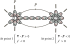
\includegraphics[scale=1]{figures/cap_02/fig_2_4.pdf}
		\caption[]{}
		\label{fig:2_4}
	\end{center}
	\vspace{-0.8cm}
\end{figure}

Let us take a spring of length $l_0$ in its undeformed state and apply the forces $\vec{F}_1$ and $\vec{F}_2$ to its ends that are equal in value and opposite in direction (\fig{2_4}). Under the action of these forces, the spring will stretch over a certain distance $\Delta l$, after which equilibrium will set in. In the state of equilibrium, the external forces $\vec{F}_1$ and $\vec{F}_2$ will be balanced by the elastic forces set up in the spring as a result of its deformation. Experiments show that with small deformations, the stretching of the spring $\Delta l$ is proportional to the stretching force: $\Delta l\propto F$ (here $F=F_1=F_2$). Accordingly, the elastic force is proportional to the elongation of the spring:
\begin{equation}\label{eq:2_25}
F = k\,\Delta l.
\end{equation}

\noindent
The constant of proportionality $k$ is called the \textbf{spring constant}.

The statement that the elastic force and deformation are proportional to each other is called \textbf{Hooke's law}.

Elastic strains are set up throughout the entire spring. Any part of the spring acts on another part with a force determined by~\eqn{2_25}. Therefore, if we cut the spring in half, an identical elastic force will appear in each half with the elongation being half the original value. Hence, we conclude that with a given material of the spring and a given coil size the magnitude of the elastic force is determined not by the absolute elongation of the spring $\Delta l$, but by its relative elongation $\Delta l/l_0$.

\begin{figure}[t]
	\begin{center}
		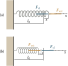
\includegraphics[scale=0.95]{figures/cap_02/fig_2_5.pdf}
		\caption[]{}
		\label{fig:2_5}
	\end{center}
	\vspace{-0.7cm}
\end{figure}

Elastic strains, but of the opposite sign, are also set up when a spring is compressed. Let us generalize~\eqn{2_25} as follows. We shall rigidly fix one end of a spring (\fig{2_5}) and shall consider the elongation of the spring as the coordinate $x$ of its other end measured from its position corresponding to the undeformed spring\footnote{In~\fig{2_5}b, the distance over which the end of the spring moved is designated $-x$. The reason is that the distance is a positive quantity, while the		coordinate $x$ in this case, however, is a negative one.}. In addition, by $F$ we shall understand the projection of the elastic force $\vec{F}_{\text{el}}$ onto the $x$-axis. We can thus write that
\begin{equation}\label{eq:2_26}
F = -k x
\end{equation}

(inspection of~\fig{2_5} shows that the projection of the elastic force onto the $x$-axis and the coordinate $x$ always have opposite signs).

%\begin{figure}[t]
%	\begin{minipage}[t]{0.5\linewidth}
%		\begin{center}
%			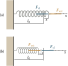
\includegraphics[scale=0.75]{figures/cap_02/fig_2_5.pdf}
%			\caption[]{}
%			\label{fig:2_5}
%		\end{center}
%	\end{minipage}
%	\hspace{-0.05cm}
%	\begin{minipage}[t]{0.5\linewidth}
%		\begin{center}
%			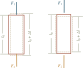
\includegraphics[scale=0.72]{figures/cap_02/fig_2_6.pdf}
%			\caption[]{}
%			\label{fig:2_6}
%		\end{center}
%	\end{minipage}
%	\vspace{-0.7cm}
%\end{figure}

Homogeneous bars behave in tension or uniaxial compression like a spring. If we apply the forces $\vec{F}_1$ and $\vec{F}_2$ ($F_1=F_2=F$) to the ends of a bar, these forces being directed along its axis and acting uniformly over the entire cross section, then the length of the bar $l_0$ will receive either a positive (in stretching) or a negative (in compression) increment\footnote{A change in the length of the bar is attended by a corresponding change in its cross-sectional dimensions.} $\Delta l$ (\fig{2_6}). It is quite natural to take the relative change in the length of the bar as the quantity characterizing its deformation:
\begin{equation}\label{eq:2_27}
\varepsilon = \frac{\Delta l}{l_0}.
\end{equation}

Experiments show that for bars of a given material the relative elongation or strain in elastic deformation is proportional to the force per unit cross-sectional area of the bar:
\begin{equation}\label{eq:2_28}
\varepsilon = \alpha\frac{\Delta l}{S}.
\end{equation}

\noindent
The constant of proportionality a is called the \textbf{compliance coefficient}.

\begin{figure}[t]
	\begin{center}
		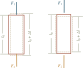
\includegraphics[scale=0.95]{figures/cap_02/fig_2_6.pdf}
		\caption[]{}
		\label{fig:2_6}
	\end{center}
	\vspace{-0.7cm}
\end{figure}

The quantity equal to the ratio between the force and the area of the surface it is acting on is called the stress. Owing to the interaction of the parts of a body with one another, the stress is transmitted to all points of the body---the entire volume of the body, for example a bar, will be in a stressed state. If the force is directed along a normal to the surface, the stress is called \textbf{normal}. If it is directed along a tangent to the surface it is acting on, the stress is called \textbf{tangential} (\textbf{shear}). The normal stress is designated by the symbol $\sigma$, the tangential or shear stress by the symbol $\tau$.

The ratio $F/S$ in~\eqn{2_28} is the normal stress $\sigma$. Hence, this equation can be written in the form
\begin{equation}\label{eq:2_29}
\varepsilon = \alpha\sigma.
\end{equation}

\noindent
In addition to the compliance coefficient $\alpha$, the elastic properties of a material are also characterized by its reciprocal $E=1/\alpha$, which is called the \textbf{modulus of elasticity} or \textbf{Young's modulus}. It is measured in pascals (the pascal is the unit of pressure in the SI system---$\SI{1}{\pascal}=\SI{1}{\newton\per\square\metre}$).

Using $1/E$ instead of $\alpha$ in~\eqn{2_9}, we get
\begin{equation}\label{eq:2_30}
\varepsilon = \frac{\alpha}{E}
\end{equation}

\noindent
from which it follows that Young's modulus equals such a normal stress at which the relative elongation or strain will equal unity (\ie, the increment of the length $\Delta l$ will be equal to the original length $l_0$) if so great elastic deformations were possible (actually a bar will fail at considerably smaller stresses, and the elastic limit is reached still earlier).

Solving~\eqn{2_28} with respect to $F$ and using $\Delta l/l_0$ instead of $\varepsilon$ and $1/E$ instead of $\alpha$, we get
\begin{equation}\label{eq:2_31}
F = \frac{E\,S}{l_0}\Delta l = k\,\Delta l
\end{equation}

\noindent
where $k$ is a constant quantity for a given bar. Equation~\eqref{eq:2_31} expresses Hooke's law for a bar [compare with~\eqn{2_26}]. Do not forget that this law is obeyed only until the elastic limit is reached. 

\begin{figure}[t]
	\begin{center}
		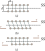
\includegraphics[scale=1]{figures/cap_02/fig_2_7.pdf}
		\caption[]{}
		\label{fig:2_7}
	\end{center}
	\vspace{-0.7cm}
\end{figure}

In conclusion, let us briefly consider shear strain. Let us take a homogeneous body having the shape of a rectangular parallelepiped and apply to its opposite faces the forces $\vec{F}_1$ and $\vec{F}_2$ ($F_1=F_2=F$) directed parallel to these faces (~\fig{2_7}). If the action of the forces is uniformly distributed over the entire surface of the corresponding face, then in any cross section parallel to these faces the tangential (shear) stress
\begin{equation}\label{eq:2_32}
\tau = \frac{F}{S}
\end{equation}

\noindent
will appear ($S$ is the area of a face). The action of the stresses will cause the body to deform so that one face will move relative to another over the distance $a$. If we mentally divide the body into elementary layers parallel to the faces we are considering, then each layer will be shifted with respect to its neighbours. For this reason, such deformation is called \textbf{shear}.

In shear, any straight line originally perpendicular to the layers will turn through the angle $\varphi$. Shear is characterized by the quantity
\begin{equation}\label{eq:2_33}
\gamma = \frac{a}{b} = \tan\varphi
\end{equation}

\noindent
called the \textbf{relative shear} (what $a$ and $b$ are is clear from~\fig{2_7}). Upon elastic deformations, the angle $\varphi$ is very small. We can therefore assume that $\tan\varphi\approx\varphi$. Consequently, the relative shear $\gamma$ equals the angle of shear $\varphi$.

Experiments show that the relative shear is proportional to the tangential stress:
\begin{equation}\label{eq:2_34}
\gamma = \frac{1}{G}\tau.
\end{equation}

\noindent
The coefficient $G$ depends only on the properties of a material and is called the \textbf{shear modulus}. It equals such a tangential (shear) stress at which the angle of shear will be 45 degrees ($\tan\varphi=1$) if the elastic limit were not exceeded at such great deformations. The shear modulus $G$, like Young's modulus $E$, is measured in pascals (\si{\pascal}).

\section{Friction Forces}\label{sec:2_10}

Forces of friction appear when contacting bodies or their parts move relative to one another. The friction occurring in the relative movement of two contacting bodies is called \textbf{external}; the friction between parts of the same continuous body (for example, a fluid) is called \textbf{internal}.

The force of friction appearing when a solid body moves relative to a fluid (liquid or gas) medium must be related to the category of internal friction forces because in this case the layers of the fluid in direct contact with the body are carried along with it at the body's velocity. The motion of the body is influenced by the friction between these layers of the fluid and other of its layers that are external relative to them.

Friction between the surfaces of two solids in the absence of any intermediate layer, for instance, a lubricant between them, is called \textbf{dry}. Friction between a solid and a fluid, and also between the layers of a fluid, is called \textbf{viscous} (or \textbf{liquid}).

Two kinds of dry friction are distinguished: \textbf{sliding} and \textbf{rolling}.

Forces of friction are directed along a tangent to the surfaces (or layers) in contact so that they resist the relative displacement of these surfaces (layers). If, for example, two layers of a liquid slide over each other with different velocities, then the force applied to the faster layer is directed oppositely to the direction of motion, while the force acting on the slower layer is directed along its motion.

\begin{figure}[t]
	\begin{center}
		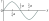
\includegraphics[scale=1]{figures/cap_02/fig_2_8.pdf}
		\caption[]{}
		\label{fig:2_8}
	\end{center}
	\vspace{-0.7cm}
\end{figure}

\textbf{Dry Friction.} In dry friction, a force of friction appears not only when one surface slides over another one, but also when attempts are made to set up such sliding motion. In the latter case, we have to do with the \textbf{force of static friction}. Let us consider two contacting bodies $1$ and $2$ of which the latter is fixed in place (\fig{2_8}). Body $1$ is pressed against body $2$ by the force $\vec{F}_{\hatvec{n}}$ directed along a normal to the surface of contact of the bodies. It is called the \textbf{normal force} and may be due to the pressure of the body's weight, or to other reasons. Let us try to move body $1$ by acting on it with an external force $\vec{F}$. We shall find that for every concrete pair of bodies and every value of the normal force there is a definite minimum value $F_0$ of the force $\vec{F}$ at which body $1$ first begins to move. At values of the external force $F$ within the limits from $0$ to $F_0$, the body remains at rest. According to Newton's second law, this is possible if the force $\vec{F}$ is balanced by a force equalling it in magnitude and opposite in direction, which is exactly the force of static friction $\vec{F}_{\text{fr}}$ (see~\fig{2_8}). It automatically\footnote{This occurs in the same way as a spring acted upon by a stretching force automatically acquires an elongation such that the elastic force balances the external one.} acquires a value equal to that of the external force $F$ (provided that the latter does not exceed $F_0$). The quantity $F_0$ is the maximum possible value of the force of static friction.

It must be noted that in accordance with Newton's third law body $2$ must also experience the force of static friction $\vec{F}_{\text{fr}}'$ (it is shown by a dashed arrow in~\fig{2_8}) equal in magnitude to the force $\vec{F}_{\text{fr}}$ but directed oppositely.

If the external force $\vec{F}$ exceeds $F_0$ in magnitude, the body begins to slide. Its acceleration is determined by the resultant of two forces: the external one $\vec{F}$ and the force of sliding friction $\vec{F}_{\text{fr}}$ whose magnitude depends to a certain extent on the sliding speed. The nature of this relation is determined by the nature and state of the contacting surfaces. The kind of the speed dependence of the force of friction shown in~\fig{2_9} is encountered most frequently. The graph shows both static and sliding friction. The force of static friction, as we have already noted, may range from $0$ to $F_0$, which is shown by the vertical line in the graph. In accordance with~\fig{2_9}, the force of sliding friction first diminishes somewhat with increasing speed, and then begins to grow. With special processing of contacting surfaces, the force of sliding friction may be virtually independent of the speed. In this case, the curved portion of the graph in~\fig{2_9} will transform into a horizontal line beginning at the point $F_0$.

\begin{figure}[t]
	\begin{center}
		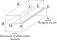
\includegraphics[scale=0.98]{figures/cap_02/fig_2_9.pdf}
		\caption[]{}
		\label{fig:2_9}
	\end{center}
	\vspace{-0.7cm}
\end{figure}

The laws of dry friction consist in the following: the maximum force of static friction, and also the force of sliding friction do not depend on the area of contact between bodies and are approximately proportional to the magnitude of the normal force pressing the contacting surfaces together:
\begin{equation}\label{eq:2_35}
F_{\text{fr}} = f\,F_{\hatvec{n}}.
\end{equation}

\noindent
The dimensionless proportionality constant $f$ is called the \textbf{coefficient of friction} (static or sliding friction, as the case may be). It depends on the nature and state of the contacting surfaces, particularly on their roughness. The coefficient of sliding friction is a function of speed.

Friction forces play a very great part in nature. Friction is often a great help to us in our everyday life. Let us remember the tremendous difficulties encountered by pedestrians and vehicles on ice-covered pavements and roads, when the friction between the pavement surface and the pedestrians' soles or the wheels of the vehicles considerably diminishes. If there were no friction forces, our furniture would have to be fastened to the floor like on a ship on a rolling sea because upon the most minute deviation of the floor from a horizontal position it would slide in the direction of the slope. Our reader can give numerous similar examples of how helpful friction is.

The part played by friction is often extremely negative, and measures have to be taken to reduce it as much as possible. This relates, for example, to the friction in bearings or between the hub of a wheel and an axle.

The most radical way of reducing forces of friction is to replace sliding friction with rolling friction. The latter appears, for example, between a cylindrical or spherical body rolling over a flat or curved surface. Rolling friction formally obeys the same laws as sliding friction, but the coefficient of friction in this case is much lower.

\textbf{Viscous Friction and Resistance of the Medium.} Unlike dry friction, viscous (internal) friction is characterized by the force of viscous friction vanishing together with the velocity. Therefore, no matter how small an external force is, it can impart a relative velocity to the layers of a viscous medium. The laws which the forces of friction between the layers of a medium obey will be considered in the chapter devoted to fluid mechanics (Chap.~\ref{chap:9}). 

\begin{figure}[t]
	\begin{center}
		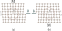
\includegraphics[scale=1]{figures/cap_02/fig_2_10.pdf}
		\caption[]{}
		\label{fig:2_10}
	\end{center}
	\vspace{-0.7cm}
\end{figure}

In this section, we shall limit ourselves to a treatment of the friction forces between a solid and a viscous (fluid) medium. It must be borne in mind that apart from the forces of friction proper, the motion of bodies in a fluid is attended by the so-called forces of \textbf{resistance of the medium} that can be much greater than the forces of friction. We have no possibility of considering the causes of these forces in detail. We shall only treat the laws obeyed jointly by forces of friction and resistance of the medium. We shall conditionally call the total force the force of friction. The speed dependence of this force is shown in~\fig{2_10}.

At low velocities, the force grows linearly with the velocity:
\begin{equation}\label{eq:2_36}
\vec{F}_{\text{fr}} = -k_1 \vec{v}
\end{equation}

\noindent
(the minus sign signifies that the force is directed oppositely to the velocity). The value of the coefficient $k_1$ depends on the shape and dimensions of a body, the state of its surface, and on the property of the fluid called its viscosity. For example, this coefficient is much higher for glycerine than for water.

At high velocities, the linear law transforms into a quadratic one, \ie, the force begins to grow in proportion to the square of the velocity:
\begin{equation}\label{eq:2_37}
\vec{F}_{\text{fr}} = -k_2\, v^2\, \vecuni{v}
\end{equation}

\noindent
($\vecuni{v}$ is the unit vector of the velocity). The value of the coefficient $k_2$ depends on the shape and dimensions of a body.

The magnitude of the velocity at which the law~\eqref{eq:2_36} transforms into~\eqref{eq:2_37} depends on the shape and dimensions of a body, and also on the viscosity and density of the fluid.

\section{Force of Gravity and Weight}\label{sec:2_11}

The force of attraction to the Earth causes all bodies to fall with the same acceleration relative to the Earth's surface, which is designated by the symbol $g$. This signifies that in a reference frame associated with the Earth, any body of mass $m$ is acted upon by the force
\begin{equation}\label{eq:2_38}
\vec{P} = m\vec{g}
\end{equation}

\noindent
called the force of gravity\footnote{Owing to the non-inertial nature of a reference frame associated with the Earth, the force of gravity will differ somewhat from the force with which a body is attracted to the Earth. This will be treated in greater detail in Sec.~\ref{sec:4_2}.}. When a body is at rest relative to the Earth's surface, the force $\vec{P}$ is balanced by the reaction\footnote{Reactions are forces with which a given body is acted upon by bodies restricting its motion.} $\vec{F}_{\text{r}}$ of the suspension or support preventing falling of the body ($\vec{F}_{\text{r}}=-\vec{P}$). According to Newton's third law, the body in this case acts on the suspension or support with the force $\vec{W}$ equal to $-\vec{F}_{\text{r}}$, \ie, with the force
\begin{equation*}
\vec{W} = \vec{P} = m\vec{g}
\end{equation*}

\begin{figure}[t]
	\begin{center}
		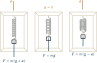
\includegraphics[scale=1]{figures/cap_02/fig_2_11.pdf}
		\caption[]{}
		\label{fig:2_11}
	\end{center}
	\vspace{-0.7cm}
\end{figure}

The force $\vec{W}$ with which a body acts on its suspension or support is called the \textbf{weight of the body}. This force equals $m\vec{g}$ only when the body and its support (or suspension) are stationary relative to the Earth. If they are moving with a certain acceleration $\vec{a}$, their weight $\vec{W}$ will not equal $m\vec{g}$. This can be explained by the following example. Let a suspension in the form of a spring fastened to a frame move together with a body with the acceleration $\vec{a}$ (\fig{2_11}). The equation of motion of the body will therefore have the form
\begin{equation}\label{eq:2_39}
\vec{P} + \vec{F}_{\text{r}} = m\vec{a}
\end{equation}

\noindent
where $\vec{F}_{\text{r}}$ is the reaction of the suspension, \ie, the force with which the spring acts on the body. According to Newton's third law, the body acts on the spring with a force equal to $-\vec{F}_{\text{r}}$, which by definition is the weight of the body $\vec{W}$ in these conditions. Substituting the force $-\vec{W}$ for the reaction $\vec{F}_{\text{r}}$ and the product $m\vec{g}$ for the force of gravity $\vec{P}$ in~\eqn{2_39}, we get
\begin{equation}\label{eq:2_40}
\vec{W} = m(\vec{g} - \vec{a}).
\end{equation}

\noindent
Equation~\eqref{eq:2_40} determines the weight of a body in the general case. It holds for a suspension or a support of any kind.

Let us assume that our body and the suspension are moving in a vertical direction (\fig{2_11} is based on this assumption).

We project~\eqn{2_40} onto the direction of a plumb line:
\begin{equation}\label{eq:2_41}
W = m(g \pm a).
\end{equation}

\noindent
In this expression, $W$, $g$, and $a$ are the magnitudes of the corresponding vectors. The plus sign corresponds to a directed upward, and the minus sign to a directed downward.

It follows from~\eqn{2_41} that the magnitude of the weight $\vec{W}$ may be either greater or smaller than the force of gravity $\vec{P}$. In free fall of the frame with the suspension, $\vec{a}=\vec{g}$, and the force $\vec{W}$ with which the body acts on the suspension vanishes. A state of weightlessness sets in. A spaceship orbiting around the Earth with its engines switched off travels, like the freely falling frame, with the acceleration $\vec{g}$. As a result, the bodies inside it are in a state of weightlessness---they exert no pressure on the bodies in contact with them.

It must be noted that the force of gravity $\vec{P}$ is often confused with the weight of a body $\vec{W}$. This is due to the fact that with a stationary support, the forces $\vec{P}$ and $\vec{P}$ coincide both in magnitude and in direction (they both equal $m\vec{g}$). It must be remembered, however, that these forces are applied to different bodies: $\vec{P}$ is applied to a body itself, whereas $\vec{W}$ is applied to the suspension or support restricting the free motion of the body in the field of the Earth's gravitational forces. In addition, the force $\vec{P}$ always equals $m\vec{g}$ regardless of whether the body is moving or at rest, whereas the force of weight $\vec{W}$ depends on the acceleration with which the support and the body are moving. It may be either greater or smaller than $m\vec{g}$, and, in particular, in a state of weightlessness it vanishes.

The relation~\eqref{eq:2_40} between the mass and the weight of a body provides a way of comparing the masses of bodies by weighing them: the ratio of the weights of bodies determined in identical conditions (usually at $\vec{a}=0$) at the same point on the Earth's surface equals the ratio of the masses of these bodies:
\begin{equation*}
W_1\,:\,W_2\,:\,W_3\,:\,\ldots = m_1\,:\,m_2\,:\,m_3\ldots.
\end{equation*}

It will be shown in Sec.~\ref{sec:4_2} that the acceleration of free fall $g$ and the force of gravity $P$ depend on the latitude of a locality. They also depend on the altitude, and diminish with an increasing distance from the centre of the Earth.

\section{Practical Application of Newton's Laws}\label{sec:2_12}

\begin{figure}[t]
	\begin{center}
		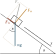
\includegraphics[scale=1]{figures/cap_02/fig_2_12.pdf}
		\caption[]{}
		\label{fig:2_12}
	\end{center}
	\vspace{-0.7cm}
\end{figure}

To compile an equation of motion, we must first of all establish what forces act on the body being considered. It is necessary to determine the action of other bodies on the given one that must be taken into account. For example, for a body sliding down an inclined plane (\fig{2_12}), the action exercised by the Earth is important (it is characterized by the force $m\vec{g}$), and also the action exercised by the plane (it is characterized by the force of the reaction $\vec{F}_{\text{r}}$).

Never take into account ``moving'', ``rolling down'', ``centripetal'', ``centrifugal''\footnote{This does not relate to the term ``centrifugal force of inertia'' (see Sec.~\ref{sec:4_2}.} and similar forces. To prevent an error, characterize a force according to the ``source'' causing it to appear, and not according to the action it produces. This means that behind every force we must see the body whose action sets up the force. This will eliminate the typical error consisting in that the same force is taken into account twice under different names.

In the example we are considering (see~\fig{2_12}), it is good to resolve the force of the reaction $\vec{F}_{\text{r}}$ into two components---the normal force $\vec{F}_{\hatvec{n}}$ and the friction force $\vec{F}_{\text{fr}}$. This, in particular, is useful in connection with the fact that the force of friction is proportional to the magnitude of the force $\vec{F}_{\hatvec{n}}$ [see~\eqn{2_35}].

Having determined the forces acting on a body, we write an equation of Newton's second law. In our example, it has the form
\begin{equation}\label{eq:2_42}
m\vec{a} = m\vec{g} + \vec{F}_{\text{r}} = m\vec{g} + \vec{F}_{\hatvec{n}} + \vec{F}_{\text{fr}}.
\end{equation}

\noindent
To perform calculations, we must pass over from vectors to their projections onto the correspondingly chosen directions, using the following properties of projections:
\begin{enumerate}[(1)]
	\item equal vectors have identical projections;
	\item the projection of a vector obtained by multiplying another vector by a scalar equals the product of the projection of this second vector and the scalar;
	\item the projection of a sum of vectors equals the sum of the projections of the vectors being added [see~\eqn{1_8}].
\end{enumerate}

Let us project the vectors in~\eqn{2_42} onto the direction $x$ shown in~\fig{2_12}. The projections of the vectors are $a_x=a$ ($a$ is the magnitude of the vector $\vec{a}$), $g_x=g\sin\alpha$, $F_{\hatvec{n}x}=0$, $F_{\text{r}x}=-f F_{\hatvec{n}x}=-fmg\cos\alpha$. Consequently, we arrive at the equation
\begin{equation*}
ma = mg\sin\alpha - fmg\cos\alpha
\end{equation*}

\noindent
from which it is a simple matter to find $a$.

In more complicated cases, we have to project the vectors onto several directions and solve the resulting system of algebraic or differential equations.
